\chapterimage{08_KoherencaB.jpg} % Chapter heading image

\chapter{Koherenca}
\label{chap:Koherenca}
Spoznali bomo koherenco, to je lastnost svetlobe, ki je tesno povezana
s pojavom interference. Obravnavali bomo časovno koherenco in zapisali 
Wiener-Hinčinov izrek ter prostorsko koherenco in z njo povezan 
Van Cittert-Zernikov izrek. Poglavje bomo zaključili z opisom holografije.

Koherenca oziroma koherentne lastnosti svetlobe se nanašajo na obstoj povezave
med fazo elektromagnetnega valovanja na nekem kraju ob nekem času ter njegovo 
fazo na nekem drugem kraju ob nekem drugem času. V poglavjih o 
uklonu (poglavje~\ref{chap:Uklon}) in interferenci (poglavje~\ref{chap:Interferenca})
smo pri zapisu elektromagnetnega valovanja privzeli, da poznamo njegovo fazo 
na vsakem kraju in ob vsakem času, s čimer smo predpostavili, 
da je elektromagnetno valovanje popolnoma koherentno. Jakost 
električnega polja popolno koherentnega valovanja zapišemo kot funkcijo $\mathbf{r}$ in $t$ 
v obliki (enačba~\ref{eq:ravnival}):
\beq
\mathbf{E} (\mathbf{r}, t) = \mathbf{E}_0(\mathbf{r}, t) 
e^{i\phi(\mathbf{r}, t)}.
\label{eq:08_01}
\eeq
Koherentno valovanje ob interferenci da značilen interferenčni 
vzorec, ki se s časom ne spreminja, nekoherentno valovanje pa ne. Pri  
delno koherentnih valovanjih interferenčne vzorce sicer opazimo, vendar z zmanjšanim
kontrastom. V realnih sistemih valovanje
ni nikoli povsem koherentno in prej ali slej se povezava med njegovo 
fazo izgubi. Ločimo časovno (tudi longitudinalno ali vzdolžno) in krajevno 
(tudi transverzalno ali prečno) koherenco. 

\section{Časovna koherenca}
Najprej bomo opisali časovno koherenco, ki povezuje valovanje na istem mestu 
ob dveh različnih časih. Za opis se omejimo na monokromatsko elektromagnetno 
valovanje v skalarnem približku. Na mestu $\mathbf{r}$ ob časih $t$ in $t+\tau$ valovanje
zapišemo kot:
\beq
E(\mathbf{r}, t) = E_0 e^{-i\omega t} e^{i\phi(\mathbf{r}, t)}
\qquad \mathrm{in} \qquad
E(\mathbf{r}, t+\tau) = E_0 e^{-i\omega (t+\tau)} e^{i\phi(\mathbf{r}, t+\tau)}.
\label{eq:08_03}
\eeq
Glede na povezavo med $\phi(\mathbf{r}, t)$ in $\phi(\mathbf{r}, t+\tau)$ 
ločimo tri vrste valovanj:
\begin{itemize}
 \item popolnoma koherentno valovanje, za katerega velja: $\phi(\mathbf{r}, t+\tau) = 
 f(\mathbf{r}, \tau, \phi(\mathbf{r}, t))$ za vsak $\tau$. 
 Če poznamo fazo valovanja ob nekem času, jo poznamo tudi ob vsakem drugem času.
 \item delno koherentno, za katerega velja:
\begin{equation}
\phi(\mathbf{r}, t)=\begin{cases}
f(\mathbf{r}, \tau, \phi(\mathbf{r}, t)); \quad \tau < \tau_c\\
\mathrm{ni~povezave}; \quad \tau > \tau_c.
\end{cases}
\label{eq:08_04}
\end{equation}
Do časa $\tau_c$, ki ga imenujemo koherenčni čas, fazo valovanja 
poznamo, pri daljših časih pa ni povezave med fazo valovanja. Večina
realnih optičnih sistemov je delno koherentnih.
 \item nekoherentno valovanje, za katerega velja, da
 sta $\phi(\mathbf{r}, t)$ in $\phi(\mathbf{r}, t+\tau)$
 povsem nepovezana in naključna za vse vrednosti $\tau$.
\end{itemize}
\begin{example}{\bf Plinska svetilka.}
Vzemimo za primer plinsko razelektritveno cev (neonsko svetilko) in 
opazujmo svetlobo, ki jo svetilka oddaja. Z uporabo barvnega 
filtra se omejimo na opazovanje ene same frekvence oziroma 
ene same spektralne komponente. Izsevana svetloba je sestavljena iz
sevalnih prispevkov vseh atomov, ki iz vzbujenega stanja prehajajo v 
nižja energijska stanja s sevanjem. V času, ki je kratek v primerjavi 
z značilnim časom med trki atomov, imajo vsa izsevana delna valovanja 
neko določeno fazo. Ob trku dveh atomov se ta faza naključno spremeni. 
Izkaže se, da je tipični čas med med trki atomov v razelektritveni cevi 
navadno le nekaj nihajnih period vidne svetlobe in shematski prikaz
izsevanega električnega polja je prikazan na sliki~\ref{fig:08_neon}.
\begin{figure}[h!]
\centering
\def\svgwidth{80truemm} 
\input{slike/08_neon.pdf_tex}
\caption{Ob trku atomov se spremeni faza izsevane svetlobe. Koherenčni
čas ocenimo kot povprečni čas med posameznimi trki.
}
\label{fig:08_neon}
\vglue-9truemm
\end{figure}

\end{example}

Časovno koherenco elektromagnetnega valovanja analiziramo z 
Michelsonovim interferometrom (glej razdelek~\ref{chap:Michelson}). 
Spomnimo se, da Michelsonov interferometer vpadni snop 
svetlobe razdeli na dva snopa, ki se nato odbijeta od zrcal in pred 
vpadom na detektor ponovno združita. Če v postavitev dodamo kolimator, 
ki iz izvorne svetlobe naredi širok vzporeden snop, dobimo tako imenovano
Twyman-Greenovo postavitev (slika~\ref{fig:08_Twyman}).
\begin{figure}[h]
\centering
\def\svgwidth{70truemm} 
\input{slike/08_TwymanGreen.pdf_tex}
\caption{Twyman-Greenova postavitev Michelsonovega interferometra. Razlika
je v kolimatorju, ki vpadno svetlobo (levo) razširi v širok snop. Snop s 
polprepustnim zrcalom razdelimo
na dva delna snopa, ki se odbijeta od zrcal, nato pa s premikanjem enega
od zrcal ustvarjamo časovni zamik med njima. Z opazovanjem 
interferenčnega vzorca svetlobe, zbrane na detektorju, določimo
koherenčni čas svetlobe.
}
\label{fig:08_Twyman}
\vglue-3truemm
\end{figure}

Vpadni snop svetlobe razdelimo na dve delni valovanji, ki po odbojih na 
zrcalih interferirata na mestu detekcije. Čeprav izvirata iz istega 
izvora, sta delni valovanji zaradi različno dolgih poti med seboj zakasnjeni. 
Časovna zakasnitev je enaka:
\beq
\tau = \frac{2 x}{c_0},
\label{eq:08_05}
\eeq
pri čemer je $x$ pomik zrcala in $2x$ razlika v dolžini poti med prvo in drugo 
vejo interferometra. 

Jakost
električnega polja na detektorju zapišemo kot vsoto dveh delnih valovanj:
\beq
E_d = E(t) + E(t+\tau).
\label{eq:08_06}
\eeq
Gostota svetlobnega toka  je sorazmerna kvadratu jakosti:
\beq
j_d \propto |E(t) + E(t+\tau)|^2 = \left(E(t) + E(t+\tau)\right) 
\left(E^*(t) + E^*(t+\tau)\right)\!,
\label{eq:08_07}
\eeq
od koder sledi:
\beq
j_d \propto |E(t)|^2 + |E(t+\tau)|^2 + E(t)E^*(t+\tau) + E^*(t)E(t+\tau).
\label{eq:08_08}
\eeq
Z detektorjem zajemamo signal v časovnem intervalu $T$, ki je bistveno 
daljši od nihajnega časa svetlobe. Zato na detektorju zaznamo povprečen signal:
\beq
\langle j_d \rangle \propto \frac{1}{T}\int_{-T/2}^{T/2} 
\left(|E(t)|^2 + |E(t+\tau)|^2 + 2 \Re \left( E(t)E^*(t+\tau)\right) \right) dt.
\label{eq:08_09}
\eeq
Kadar sta amplitudi delnih žarkov enaki, velja:
\beq
\langle j_d \rangle \propto 2\langle |E(t)|^2 \rangle + 2\frac{1}{T}\int_{-T/2}^{T/2} 
\Re \left( E(t)E^*(t+\tau)\right) dt.
\label{eq:08_10}
\eeq
Vpeljemo časovno avtokorelacijsko funkcijo periodičnega polja za dolge čase zajemanja:
\boxeq{eq:G1}{
G^{(1)}(\tau)= \lim_{T\to \infty}~\frac{1}{T}\int_{-T/2}^{T/2}E(t)E^*(t+\tau)dt
}
in signal na detektorju zapišemo kot:
\beq
\langle j_d \rangle \propto 2\langle |E(t)|^2 \rangle + 
2\Re \left( G^{(1)}(\tau)\right)\!\!.
\label{eq:08_11}
\eeq
Zapisana avtokorelacijska funkcija podaja korelacijo valovanja samega s seboj pri
dani časovni zakasnitvi $\tau$. Poglejmo nekaj primerov.

\begin{example}{\bf Avtokorelacija sinusnega valovanja.}
Obravnavajmo ravno sinusno elektromagnetno valovanje pri točno določeni frekvenci. 
Zapišemo ga v obliki:
\beq
E(t) = E_0 e^{-i\omega_0 t} \qquad \mathrm{in} \qquad E(t+\tau)= E_0 e^{-i\omega_0(t+\tau)},
\label{eq:08_12}
\eeq
pri čemer je $E_0$ realno število. Potem je časovna avtokorelacijska 
funkcija (enačba~\ref{eq:G1}) enaka:
\beq
G^{(1)}(\tau) = \lim_{T\to \infty}~\frac{1}{T}
\int_{-T/2}^{T/2}E_0 e^{-i\omega_0 t}E_0^*e^{i\omega_0 t}e^{i\omega_0\tau} dt.
\label{eq:08_13}
\eeq
Sledi:
\beq
G^{(1)}(\tau) = E_0^2 e^{i\omega_0 \tau} 
\lim_{T\to \infty}~\frac{1}{T}\int_{-T/2}^{T/2} dt= E_0^2 e^{i\omega_0 \tau}.
\label{eq:08_14}
\eeq
Če se omejimo zgolj na realni del, velja:
\beq
G^{(1)}(\tau) = E_0^2 \cos(\omega_0 \tau).
\label{eq:08_14a}
\eeq
Gostota svetlobnega toka na detektorju je potem enaka (enačba~\ref{eq:08_11}):
\beq
\langle j_d \rangle \propto  
2E_0^2 + 2 E_0^2 \cos(\omega_0 \tau).
\label{eq:08_15}
\eeq
Vpeljemo $j_0$ kot gostoto energijskega toka posameznega delnega valovanja 
in izmerjeno  gostoto toka na detektorju preoblikujemo v:
\beq
\langle j_d \rangle  = 4j_0 \cos^2\frac{\omega_0 \tau}{2}.
\label{eq:08_15a}
\eeq
Signal na detektorju je prikazan na sliki~\ref{fig:08_sinkoh}\,a.
Z uporabo enačbe~(\ref{eq:08_05}) preoblikujemo še argument funkcije:
\beq
\frac{\omega_0 \tau}{2} = \omega_0 \frac{x}{c_0} = k x = \frac{\Delta \phi}{2}.
\label{eq:08_17}
\eeq
Dobimo izraz:
\beq
\langle j_d \rangle  = 4j_0 \cos^2 (\Delta \phi/2).
\label{eq:08_15c}
\eeq
ki ga že poznamo iz poglavja o interferenci (enačba~\ref{eq:06_09}). 

Zapisani rezultat velja samo v primeru povsem koherentnega monokromatskega 
sinusnega valovanja, za katerega znamo zapisati fazo v vsakem trenutku. 
V praksi opisano obnašanje opazimo le v bližini ekvidistančne 
lege zrcal za majhne vrednosti $\Delta \phi$. Ko razliko v poteh posameznih delnih 
žarkov povečujemo, se koherenca valovanja zmanjšuje in kontrast interferenčnega vzorca bledi 
(slika~\ref{fig:08_sinkoh}\,b).
Pri zelo velikih vrednostih $x$ imata delna žarka naključni fazi, 
kar pomeni, da $\Delta \phi$ zavzema naključne vrednosti med $0$ in $2\pi$. 
Posledično je povprečje $\langle \cos \Delta \phi \rangle= 0$
in za velike vrednosti $\tau$ velja:
\beq
\langle j_d \rangle = 2 j_0.
\label{eq:08_18}
\eeq
\begin{figure}[h]
\vglue-3truemm
\centering
\def\svgwidth{140truemm} 
\input{slike/08_sinkoh.pdf_tex}
\caption{Signal na detektorju Michelsonovega interferometra v odvisnosti od premika zrcala $x$
v primeru koherentnega monokromatskega sinusnega valovanja (a). Kadar je dolžina valovanja
končna in valovanje ni povsem monokromatsko, kontrast signala pri večjih $x$ oslabi.
Karakteristična razdalja, na kateri kontrast signala oslabi, je koherenčna dolžina $L_c = c \tau_c$.
}
\label{fig:08_sinkoh}
\vglue-7truemm
\end{figure}

\end{example} 

\begin{example}{\bf Avtokorelacija dušenega valovanja.}
Izračunajmo avtokorelacijsko funkcijo eksponentno pojemajočega polja, ki ga zapišemo
v obliki:
\beq
E(t) = E_0 e^{-t/\tau_0}e^{-i\omega_0 t}.
\label{eq:08_101}
\eeq
Za razliko od prejšnjega primera, pri katerem je bil signal periodična funkcija in njegovo 
trajanje bistveno daljše od časa merjenja $T$, moramo za neperiodične funkcije avtokorelacijsko
funkcijo vpeljati drugače. Zapišemo:
\boxeq{eq:G12}{
\tilde{G}^{(1)}(\tau)= \int_{-\infty}^{\infty}E(t)E^*(t+\tau)dt.
}
Pri periodičnih funkcijah je namreč smiselno govoriti o povprečni vrednosti, pri neperiodičnih, 
kot sta na primer eksponentno pojemajoča funkcija ali kratek sunek Gaussove oblike, pa ne. 
Ustrezno postavimo tudi meje integracije, pri Gaussovem sunku, na primer, od $-\infty$ do $\infty$, 
pri eksponentno pojemajoči funkciji pa od $0$ do $\infty$. Avtokorelacijska 
funkcija polja (enačba~\ref{eq:08_101}) je potem:
\beq
\tilde{G}^{(1)}(\tau)= \int_{0}^{\infty}E_0^2 e^{-t/\tau_0}e^{-i\omega_0 t}
e^{-(t+\tau)/\tau_0}e^{i\omega_0 (t+\tau)} dt = E_0^2 e^{i\omega_0 \tau}e^{-\tau/\tau_0} 
\int_{0}^{\infty} e^{-2t/\tau_0}dt.
\label{eq:08_103}
\eeq
Sledi:
\beq
\tilde{G}^{(1)}(\tau)= E_0^2 \frac{\tau_0}{2}e^{-\tau/\tau_0}e^{i\omega_0 \tau}.
\label{eq:08_104}
\eeq
Avtokorelacijska funkcija eksponentno pojemajočega polja je eksponentno pojemajoča funkcija.
Podobno kratek račun pokaže, da je avtokorelacijska funkcija sunka svetlobe Gaussove oblike 
prav tako Gaussova funkcija. 
\end{example}

Namesto koherenčnega časa $\tau_c$ lahko vpeljemo koherenčno dolžino 
$L_c = c_0 \tau_c$, ki označuje pot, ki jo svetloba prepotuje 
v koherenčnem času. Časovno koherenco zato imenujemo tudi 
longitudinalna ali vzdolžna koherenca, saj opazujemo zamik valovanja, ki se
premakne vzdolžno glede na smer širjenja svetlobe. Valovanje, ki je 
koherentno za $\tau < \tau_c$, je tako pri opisanem eksperimentu 
koherentno za spremembe dolžine poti, za katere velja $L < L_c$. Pri 
večjih razlikah v dolžini poti se koherenca zmanjša in kontrast
interferenčne slike izgubi. 

\section{Wiener-Hinčinov izrek}
Michelsonov interferometer lahko uporabimo za meritve emisijskih spektrov svetil
ali absorpcijskih spektrov snovi. Takrat svetloba, ki vpada na interferometer,
ni monokromatska, ampak je sestavljena iz valovanj z različnimi valovnimi dolžinami.
S premikanjem zrcala interferometra na detektorju posnamemo celoten interferogram. Pokazali bomo, da
spekter vpadne svetlobe izračunamo kot Fourierevo transformiranko posnetega interferograma. 

Najprej razstavimo periodično vpadno električno polje na posamična valovanja z diskretnim
Fourierevim razvojem. Pri tem upoštevamo, da polje analiziramo in zaznavamo le v nekem končnem
časovnem intervalu $T$. Fourierev razvoj je potem:
\beq
E(t) = \sum_n A_n e^{-i n \Delta\omega t},
\label{eq:08_19}
\eeq
pri čemer je širina intervala $\Delta\omega = 2\pi/T$, $n$ pa je celo število. Koeficienti
razvoja $A_n$ označujejo delež polja pri krožni frekvenci $n\Delta \omega$. 
V nadaljevanju bomo krožno frekvenco posamezne komponente pisali kot 
$\omega_n$:
\beq
\omega_n = n \Delta \omega = n \frac{2\pi}{T}.
\label{eq:08_20}
\eeq
Razstavimo še polje zakasnjenega delnega valovanja oziroma njegove kompleksno konjugirane vrednosti:
\beq
E^*(t+\tau) = \sum_m A_m^* e^{i\omega_m (t + \tau)},
\label{eq:08_21}
\eeq
kjer je $m$ celo število. Signal na detektorju je sorazmeren z avtokorelacijsko funkcijo
polja, zato razstavljeni polji vstavimo v definicijo avtokorelacijske funkcije (enačba~\ref{eq:G1}):
\beq
G^{(1)}(\tau) = \lim_{T\to\infty} \frac{1}{T} \int_{-T/2}^{T/2} \sum_{n,m} A_n A_m^* e^{-i\omega_n t}
e^{i\omega_m (t+\tau)} dt.
\label{eq:08_22}
\eeq
Sledi:
\beq
G^{(1)}(\tau) = 
\sum_{n,m} A_n A_m^*e^{i\omega_m\tau} \left(
\lim_{T\to\infty} \frac{1}{T} \int_{-T/2}^{T/2}e^{i(\omega_m - \omega_n)t}dt \right)\!\!.
\label{eq:08_23}
\eeq
Privzamemo, da je čas meritve razmeroma dolg ($T\to\infty$) in izraz v oklepaju zapišemo kot funkcijo
$\delta(\omega_n - \omega_m)$. Dobimo:
\beq
G^{(1)}(\tau) = \sum_m|A_m|^2e^{i\omega_m\tau}.
\label{eq:08_24}
\eeq 
Izračunajmo Fourierevo transformiranko avtokorelacijske funkcije:
\beq
\frac{1}{2\pi}\int_{-\infty}^{\infty} G^{(1)} (\tau) e^{-i\omega \tau} d\tau = 
\frac{1}{2\pi}\sum_m |A_m|^2 \int_{-\infty}^{\infty} e^{i\omega_m\tau}e^{-i\omega \tau} d\tau = 
\frac{T}{2\pi}|A (\omega)|^2.
\label{eq:08_25}
\eeq
V zadnjem koraku smo upoštevali enačbo~(\ref{eq:08_20}) in integral zapisali kot 
$T \delta (2\pi m  - \omega T)$, od koder sledi pogoj $\omega_m = \omega$. 
Spomnimo se, kaj opisujejo parametri $A(\omega)$: to so deleži električnega polja pri 
dani frekvenci $\omega$, kvadrat $|A(\omega)|^2$ pa je enak intenziteti svetlobe pri tej
frekvenci.

Vpeljemo spekter svetlobe $S(\omega)$ kot intenziteto svetlobe pri $\omega$ na frekvenčni 
interval $\Delta \omega$:
\beq
S(\omega) = \frac{|A(\omega)|^2}{\Delta \omega} = \frac{T}{2\pi}|A(\omega)|^2.
\label{eq:08_26}
\eeq

Primerjava enačb~(\ref{eq:08_25}) in (\ref{eq:08_26}) pokaže, da je spekter svetlobe enak 
Fourierevi transformiranki avtokorelacijske funkcije svetlobnega električnega polja:
\boxeq{eq:WH}{
S(\omega) = \frac{1}{2\pi}\int_{-\infty}^{\infty} G^{(1)} (\tau) e^{-i\omega \tau} d\tau.
}
Zapisano zvezo imenujemo Wiener-Hinčinov izrek po ameriškem matematiku Norbertu
Wienerju (1894--1964) in ruskemu matematiku Aleksandru Jakovljeviču Hinčinu (1894--1959).

Z Michelsonovim interferometrom lahko z uporabo Wiener-Hinčinovega izreka izmerimo
spekter svetlobe. Pri tem je pomembno, da signal na detektorju merimo oziroma
povprečimo čim dlje. Predvsem mora veljati $T \gg \tau_c$, sicer sploh ne bi zaznali 
preskoka faze, temveč bi izmerili navidez povsem koherentno svetlobo. 

Poleg tega smo pri računu privzeli, da poznamo avtokorelacijsko funkcij $G^{(1)}(\tau)$ 
za vse vrednosti $\tau$, to je za vse premike zrcala $x$. Tega seveda eksperimentalno
ne moremo narediti, vendar navadno velja, da so vrednosti
avtokorelacijske funkcije znatno večje od 0 le za $\tau <\tau_c$, izven merilnega
območja pa so tako majhne, da na rezultat ne vplivajo.

\begin{example}{\bf Spekter ravnega valovanja.}
Za primer si oglejmo spekter povsem koherentnega ravnega valovanja, ki ga zapišemo
kot:
\beq
E(t) = E_0 e^{-i\omega_0 t}.
\label{eq:08_27}
\eeq
Avtokorelacijsko funkcijo takega valovanja smo že izračunali (enačba~\ref{eq:08_14}), zdaj
pa izračunajmo še spekter kot Fourierevo transformacijo avtokorelacijske funkcije:
\beq
S(\omega) = \frac{1}{2\pi}\int_{-\infty}^{\infty} E_0^2 e^{i\omega_0 \tau} e^{-i\omega \tau} d\tau,
\label{eq:08_201}
\eeq
od koder sledi:
\beq
S(\omega) \propto \delta (\omega - \omega_0).
\label{eq:08_202}
\eeq
Po pričakovanju je spekter ravnega valovanja neskončno ozek (funkcija delta) pri krožni
frekvenci valovanja $\omega_0$ (slika~\ref{fig:08_spekter}\,a in b).
\end{example}

\begin{example}{\bf Spekter omejenega ravnega valovanja.}
Poglejmo še bolj realistični primer, v katerem je valovanje časovno omejeno. Naj bo 
valovanje enako ravnemu valovanju zgolj v intervalu dolžine $\tau_0$, sicer naj bo jakost
električnega polja enaka nič (slika~\ref{fig:08_spekter}\,c).
Ker gre za neperiodični signal, zapišemo avtokorelacijsko
funkcijo z enačbo~(\ref{eq:G12}), nato pa izračunamo njeno Fourierevo transformacijo.
Ker je avtokorelacijska funkcija polja konvolucija funkcije same s seboj, 
je Fouriereva transformiranka avtokorelacijske funkcije enaka kvadratu Fouriereve transformiranke
polja. Za izračun spektra moramo tako samo izračunati Fourierevo transformiranko signala:
\beq
S(\omega) = |F\{E(t)\}|^2,
\label{eq:08_203}
\eeq
pri čemer $F\{f\}$ označuje Fourierevo transformiranko funkcije $f$. Omenimo še, da je spekter
za časovno omejene signale definiran drugače kot za periodične signale. Pri periodičnih računamo
svetlobno moč na enoto frekvenčnega intervala, pri neperiodičnih pa energijo. 

Izračunati moramo torej Fourierevo transformiranko signala, ki je znotraj intervala $\tau_0$ 
enak ravnemu valovanju, sicer je enak nič:
\beq
F\{E(t)\} = \frac{1}{2\pi}\int_{-\tau_0/2}^{\tau_0/2} \cos(\omega_0 t) e^{-i\omega t} dt=
\frac{1}{2\pi}\int_{-\tau_0/2}^{\tau_0/2} \left(e^{i\omega_0 t}+ e^{-i\omega_0 t}\right)  e^{-i\omega t} dt.
\label{eq:08_204}
\eeq
Integrala izračunamo in dobimo:
\beq
F\{E(t)\} = \frac{1}{2\pi}\frac{\tau_0}{2}\left(\mathrm{sinc} \left((\omega-\omega_0)\frac{\tau_0}{2} \right)+
\mathrm{sinc} \left((\omega+\omega_0)\frac{\tau_0}{2} \right) \right),
\label{eq:08_205}
\eeq
pri čemer smo za zapis uporabili funkcijo $\mathrm{sinc}(x) = \sin(x)/x$. Kadar je dolžina sunka 
velika v primerjavi s periodo valovanja v sunku ($\omega_0\tau_0 \gg1$), 
se funkciji $\mathrm{sinc}$ pri $\pm\omega_0$ ne 
prekrivata. Takrat za spekter pri pozitivnih frekvencah velja:
\beq
S(\omega) \propto \mathrm{sinc}^2\left(\left(\omega - \omega_0\right)\frac{\tau_0}{2}\right).
\label{eq:08_206}
\eeq
Spekter je prikazan na sliki~\ref{fig:08_spekter}\,d. Ničli okoli osrednjega vrha 
spektra sta pri $\omega_0 \pm 2\pi/\tau_0$, zato širino spektra ocenimo
na $\Delta \omega = 2\pi/\tau_0$. Z naraščajočim $\tau_0$ se spekter oži in v limiti 
neskončno dolgega trajanja sunka po pričakovanju
preide v funkcijo delta pri frekvenci $\omega_0$. 
\begin{figure}[h]
\centering
\def\svgwidth{120truemm} 
\input{slike/08_spekter.pdf_tex}
\caption{Neomejenemu ravnemu valovanju (a) pripada spekter v obliki funkcije delta (b). Kadar je 
sunek valovanja končnen (c), se spekter razširi (d).
}
\label{fig:08_spekter}
\vglue-4truemm
\end{figure}

\end{example}

Na primeru smo spoznali, da je spekter povsem koherentne monokromatske svetlobe funkcija delta, 
za časovno omejene sunke pa je širina spektra obratno sorazmerna z dolžino trajanja sunka. Na splošno
velja:
\boxeq{eq:spkor}{
\Delta \omega \tau_c \gtrsim 2\pi.
}
Svetloba s kratkim koherenčnim časom ima tako širok spekter in obratno. Bela svetloba s spektralno
širino, ki ustreza $\Delta \lambda \sim 300~\si{nm}$, ima koherenčni čas $\tau_c \sim 3~\si{\femto\second}$
in koherenčno dolžino $L_c \sim 1~\si{\micro\meter}$. Z belo svetlobo tako zelo težko
izvajamo interferenčne poskuse, saj znaša koherenčna dolžina le okoli dve valovni dolžini svetlobe.
Po drugi strani z laserji s spektralno širino $\Delta \omega \sim 10~\si{kHz}$ 
dosegamo koherenčne dolžine več $100~\si{km}$. 

\section{Prostorska koherenca}
V prejšnjem razdelku smo spoznali časovno koherenco, ki opisuje povezavo
med fazo valovanja ob različnih časih. Ker časovni zamik ustreza premiku valovanja
vzdolž smeri širjenja svetlobe, časovno koherenco imenujemo tudi vzdolžna koherenca. Opazujemo
jo prek interference z delitvijo amplitude, na primer z Michelsonovim interferometrom. 

Zdaj se osredotočimo na prostorsko koherenco, ki opisuje povezavo med fazo valovanja
na različnih krajih. Ker se faza spreminja predvsem v prečni smeri, prostorsko
koherenco imenujemo tudi prečna ali transverzalna koherenca. 
Pomembna je pri interferenčnih pojavih z delitvijo valovne fronte. 
\begin{figure}[h]
\centering
\def\svgwidth{140truemm} 
\input{slike/08_kohprimer.pdf_tex}
\caption{Primerjava različnih koherenc: povsem koherentno valovanje (a), prostorsko in 
ne časovno koherentno valovanje (b), časovno in ne prostorsko koherentno valovanje (c) ter
niti časovno niti prostorsko koherentno valovanje (d).
}
\label{fig:08_kohprimer}
\vglue-4truemm
\end{figure}

Pri prostorski koherenci nas zanima faza valovanja na dveh različnih krajih $\mathbf{r}_1$ 
in $\mathbf{r}_2$ ob času $t$. Kadar sta fazi valovanja na obeh krajih povezani in velja:
\beq
\phi(\mathbf{r}, t) =  f(\mathbf{r}_2-\mathbf{r}_1, t, \phi(\mathbf{r}_1, t)),
\label{eq:08_28}
\eeq
pravimo, da sta točki $\mathbf{r}_1$ in $\mathbf{r}_2$ na isti koherenčni ploskvi. Če pa
fazi $\phi(\mathbf{r}_1, t)$ in $\phi(\mathbf{r}_2, t)$ med seboj nista povezani, ležita
na različnih koherenčnih ploskvah. 

Prostorsko koherenco analiziramo z Youngovim eksperimentom (glej poglavje~\ref{chap:Young}),
pri katerem svetlobo usmerimo na objektni zaslon z dvema majhnima odprtinama in opazujemo 
interferenčno sliko na oddaljenem zaslonu. Svetilo, s katerega vpada svetloba na odprtini,
naj bo razsežno. Ko sta odprtini v objektnem zaslonu zelo blizu skupaj, na oddaljenem zaslonu 
nastane značilna interferenčna slika. S povečevanjem razmika med odprtinama se kontrast 
interference na zaslonu zmanjšuje. Ko popolnoma zbledi, je razmik med odprtinama enak 
prečni koherenčni razdalji vpadnega valovanja. 
Zaradi preprostosti se omejimo na ravninski primer in odprtini obravnavajmo kot ozki reži.
Označimo velikost svetila z $L$, razmik med režama z $D$, oddaljenost med 
svetilom in objektnim zaslonom pa naj bo $z_0'$. Svetloba po prehodu skozi reži 
vpade na opazovalni zaslon na oddaljenosti $z_0$ od objektnega zaslona (slika~\ref{fig:08_kohprost}).
\begin{figure}[h]
\centering
\def\svgwidth{120truemm} 
\input{slike/08_kohprost.pdf_tex}
\caption{Z Youngovim poskusom analiziramo prečno koherenco svetila. S večanjem razmika med
režama $D$ se kontrast interferenčne slika na opazovalnem zaslonu spreminja. Razmik med režama,
pri katerem interferenčni vzorec izgine, določa prečno koherenčno razdaljo. Privzamemo, da 
velja $D \ll z_0, z_0'$.
}
\label{fig:08_kohprost}
\vskip-4truemm
\end{figure}

Žarki, ki izhajajo iz ene točke svetila, med seboj interferirajo, v primeru razsežnega svetila
pa na zaslonu opazujemo superpozicijo interferenčnih vzorcev z različnih 
delov svetila. Na opazovalnem zaslonu si izberemo točko, ki je simetrična glede na odprtini 
v objektnem zaslonu. Potem sta fazi žarkov, ki 
izhajata s sredine svetila, enaki, medtem ko se fazi žarkov, ki izhajata z roba svetila, 
razlikujeta za 
\beq
\Delta \phi = k D \sin \beta \approx kD \frac{L}{2z_0'}.
\label{eq:08_29}
\eeq
S spreminjanjem razmika med režama se fazni zamik med žarkoma z roba svetila povečuje. 
Ko doseže $\pi$, je signal z roba svetila v protifazi signalu s sredine svetila in 
interferenčna slika na zaslonu izgine. Zapišemo:
\beq
\pi = \frac{2\pi}{\lambda}D_c\frac{L}{2z_0'},
\label{eq:08_30}
\eeq
od koder sledi:
\boxeq{eq:08_31}{
D_c= \frac{z_0'\lambda}{L}.
}
Razdalja med režama $D_c$, pri kateri interferenčni vzorec izgine oziroma se signal izpovpreči, 
določa transverzalno koherenčno razdaljo svetlobe, ki vpada na objektni zaslon. Parameter $D_c^2$
je merilo za velikost koherenčne ploskve vpadne svetlobe. 
\begin{remark}
\vglue-6truemm
Zapisali smo, da pri večanju razmika med režami fazni zamik med žarkoma, ki vpadata na zaslon skozi
prvo in drugo režo, narašča. Zato bi pričakovali, da se pri faznem zamiku, ki je večji od $\pi$,
kontrast povečuje. Vendar je bil račun narejen samo za dva žarka. Kadar upoštevamo prispevke
vseh delov svetila, se izkaže, da je kontrast za vse razmike, ki so večji od $D_c$, praktično enak nič.
\vglue-6truemm
\end{remark}

Koherenčno razdaljo lahko zapišemo tudi kot funkcijo zornega kota $\alpha$, to je kota, pod 
katerim opazujemo oddaljen predmet:
\beq
D_c = \frac{\lambda}{\alpha}.
\label{eq:08_32}
\eeq
Kadar je zorni kot zelo majhen, je koherenčna ploskev velika. Ta odvisnost se izraža na primer
pri oddaljenih zvezdah. Zvezde so sicer velike in oddajajo nekoherentno svetlobo, vendar je 
zaradi velike oddaljenosti in posledično majhnega zornega kota svetloba, ki vpada 
na teleskope, prostorsko koherentna.

\begin{example}{\bf Merjenje velikosti zvezd.}
Z Youngovim poskusom lahko izmerimo velikost zvezde, če poznamo njeno oddaljenost. 
Ker zvezde opazujemo pod zelo majhnim zornim kotom, je njihova koherenčna ploskev
na Zemlji razmeroma velika. Zato namesto premičnih odprtin v zaslonu uporabimo dve 
premični zrcali, ki vpadno svetlobo prek drugega para zrcal usmerita na zbiralno lečo.
Na zaslonu opazujemo interferenco valovanj, ki vpadata pod malenkost različnima vpadnima kotoma
(slika~\ref{fig:08_Stellar}). Z večanjem razmika med zrcaloma interferenčni kontrast izgine, kar
omogoča določiti velikost zvezde.
\begin{figure}[h]
\centering
\def\svgwidth{80truemm} 
\input{slike/08_Stellar.pdf_tex}
\caption{Michelsonov zvezdni interferometer, s katerim merimo velikost zvezd. 
Z večanjem razmika med zrcaloma ($D$) kontrast na zaslonski sliki izgine in iz razmika med zrcaloma 
lahko določimo zorni kot zvezde.}
\label{fig:08_Stellar}
\end{figure}

Z opisano postavitvijo sta leta 1920 Michelson in astronom Francis Gladheim Pease
prvič izmerila premer katerekoli zvezde. Opazovala sta interferenco svetlobe z 
zvezde $\alpha$ v ozvezdju Orion (Betelgeza) in opazila, da pri razmiku zrcal, večjem
od $D_c = 307~\si{cm}$, interferenčni kontrast izgine. Privzela sta, da je valovna dolžina
svetlobe $575~\si{nm}$ in z upoštevanjem popravka za okrogel predmet (glej enačbo~\ref{eq:05_42}) 
določila zorni kot:
\beq
\alpha = 1,22 \frac{\lambda}{D_c} = 2,3 \times 10^{-7}~\si{\radian} = 0,047\si{\arcsec}.
\label{eq:08_33}
\eeq
Z upoštevanjem oddaljenosti zvezde (podatek so pridobili iz paralakse) sta ocenila premer
na $390 \times 10^6~\si{km}$, kar ustreza približno $300~\times$ premeru Sonca. Poznejše 
natančnejše meritve so pokazale, da je zvezda približno trikrat večja. Glavnina napake je 
izvirala iz nenatančne ocene oddaljenosti zvezde. 
\end{example}

\section{Van Cittert-Zernikov izrek}
Obravnavajmo prostorsko koherenco podrobneje. Pokazali bomo, da je kontrast interferenčnih prog
na zaslonu sorazmeren z navzkrižno korelacijsko funkcijo jakosti električnega polja, podobno kot
je pri časovni koherenci kontrast interferenčnih prog sorazmeren z avtokorelacijsko funkcijo polja
(enačba~\ref{eq:G12}). Nadalje velja, da je kontrast interferenčnih prog sorazmeren z 2D-Fourierevo
transformiranko intenzitetne porazdelitve na oddaljenem izvoru. Čeprav je svetloba, ki jo oddaja
svetilo, nekoherentna, stopnja njene koherence narašča z oddaljenostjo, zato je svetloba, ki vpada z zelo
oddaljenih svetil (na primer zvezd), koherentna. Z inverzno transformiranko lahko iz izmerjenega
interferenčnega vzorca določimo intenzitetno porazdelitev svetila. To ugotovitev imenujemo
Van Cittert-Zernikov izrek po nizozemskem fiziku Pietru Hendriku van Cittertu (1889-1959) 
in nizozemskem fiziku in nobelovcu Fritsu Zerniku (1888--1966).

Naj svetloba s svetila vpada na objektni zaslon, v katerem sta dve odprtini, na oddaljenem
opazovalnem zaslonu pa opazujemo interferenčno sliko (slika~\ref{fig:08_VCZ}). Svetloba, ki vpada 
na dano točko zaslona, je sestavljena iz prispevkov iz prve in druge odprtine. Privzamemo, 
da je meritev dovolj dolga, da z detektorjem zaznavamo povprečni signal $\langle j_d \rangle$.
\begin{figure}[h]
\centering
\def\svgwidth{110truemm} 
\input{slike/08_VCZ.pdf_tex}
\caption{Svetloba iz nekoherentnega izvora vpada na objektni zaslon, v katerem sta dve odprtini.
Na oddaljenem objektnem zaslonu opazujemo interferenčno sliko v odvisnosti od razmika med 
odprtinami. Ko razmik doseže koherenčno razdaljo, kontrast interferenčnih prog izgine.}
\label{fig:08_VCZ}
\vskip-4truemm
\end{figure}

Povprečni signal na detektorju je sorazmeren kvadratu jakosti električnega polja, ki ga zapišemo
kot vsoto prispevkov iz posameznih odprtin:
\beq
\langle j_d \rangle \propto \langle|E_1(t)+ E_2(t+\tau)|^2 \rangle,
\label{eq:08_34}
\eeq
pri čemer smo upoštevali časovni zamik $\tau$, ki nastane zaradi različno dolgih poti od
odprtin do detektorja. Sledi:
\beq
\langle j_d \rangle \propto \langle|E_1(t)|^2 \rangle + \langle|E_2(t+\tau)|^2 \rangle
+ 2\Re \left( \frac{1}{T}\int_{-T/2}^{T/2}E_1(t)E_2^*(t+\tau) dt \right)\!\!.
\label{eq:08_35}
\eeq
Pri tem prvi člen opisuje svetlobno polje iz prve reže, drugi člen svetlobo iz druge reže, 
izraz v oklepaju tretjega člena pa predstavlja navzkrižno korelacijsko funkcijo polja ob dolgih
časih meritve:
\boxeq{eq:CC}{
\Gamma_{12}(\tau) = \lim_{T\to \infty}\frac{1}{T}\int_{-T/2}^{T/2}E_1(t)E_2^*(t+\tau) dt.
}
Kadar je svetloba iz 
posamezne reže časovno koherentna, velja:
\beq
E^*(t+\tau) = e^{i \omega \tau} E^*(t)
\label{eq:08_36}
\eeq
in navzkrižno korelacijsko funkcijo zapišemo kot:
\beq
\Gamma_{12}(\tau) = e^{i \omega \tau} \frac{1}{T}\int_{-T/2}^{T/2}E_1(t)E_2^*(t) dt =
 J_{12} e^{i \omega \tau}. 
 \label{eq:08_37}
\eeq
Člen $J_{12}$, ki je enak:
\beq
J_{12} = \frac{1}{T}\int_{-T/2}^{T/2}E_1(t)E_2^*(t) dt,
\label{eq:08_38}
\eeq
je odvisen od prostorske koherence valovanja in določa kontrast oziroma vidljivost interferenčne slike
na opazovalnem zaslonu. Zaradi preglednosti v zapisu izpuščamo limito, vendar se moramo zavedati, 
da zapisano velja le za dovolj dolge meritve.

Označimo z $(x_1, y_1)$ koordinate prve odprtine v objektnem zaslonu in z $(x_2, y_2)$
koordinate druge odprtine. Svetilo s ploskvijo $S$ naj leži v ravnini $x'y'$. Potem je svetloba, 
ki vpada na posamezno odprtino, sestavljena iz prispevkov vseh točk svetila $S$. Polje v prvi
odprtini zapišemo kot:
\beq
E_1 \propto \iint_S E_0(x',y') \frac{e^{ikr_1'}}{r_1'}dx'dy'
\label{eq:08_39}
\eeq
in podobno polje v drugi reži kot:
\beq
E_2 \propto \iint_S E_0(x'',y'') \frac{e^{ikr_2''}}{r_2''}dx''dy''.
\label{eq:08_40}
\eeq
Vstavimo polji v enačbo~(\ref{eq:08_38}) in dobimo:
\beq
J_{12} \propto \iint_S \iint_S \langle E_0(x',y') E_0^*(x'',y'') \rangle  \frac{e^{ik(r_1'-r_2')}}{r_1'r_2'}dx'dy'dx''dy''.
\label{eq:08_41}
\eeq
Kadar je svetloba, ki izvira iz različnih delov svetila med seboj povsem nekorelirana,
je povprečje različno od nič le v primeru, ko sta $x'=x''$ in $y'=y''$. To seveda velja, 
če svetilo samo po sebi ni prostorsko koherentno, denimo termična svetloba zvezd.
Zapišemo:
\beq
\langle E_0(x',y') E_0^*(x'',y'') \rangle \propto \delta(x'-x'', y'-y'') |E_0(x',y')|^2.
\label{eq:08_42}
\eeq
Enačbo~(\ref{eq:08_41}) poenostavimo, pri čemer privzamemo, da je oddaljenost svetila od 
objektnega zaslona bistveno večja od dimenzij svetila, tako da $r_1'$ in $r_2'$ v imenovalcu 
nadomestimo z $z_0'$:
\beq
J_{12} \propto \iint_S |E_0(x',y')|^2 \frac{e^{ik(r_1'-r_2')}}{z_0'^2}dx'dy'
\propto \frac{1}{z_0'^2}\iint_S j_0(x',y') e^{ik(r_1'-r_2')}dx'dy'.
\label{eq:08_43}
\eeq
Z $j_0(x',y')$ smo označili intenziteto svetlobe, ki jo oddaja izbrana točka na svetilu, 
v odvisnosti od lege točke $(x',y')$.

Parameter $r_1'$ razvijemo za veliko oddaljenost izvora od objektnega zaslona:
\beq
r_1' = \sqrt{z_0'^2+(x_1-x')^2+ (y_1-y')^2} \approx
z_0'-\frac{x_1x'}{z_0'}-\frac{y_1y'}{z_0'}+\frac{x_1^2}{2z_0'}+\frac{y_1^2}{2z_0'}+\frac{x'^2}{2z_0'}
+\frac{y'^2}{2z_0'}.
\label{eq:08_44}
\eeq
Ter podobno za drugo odprtino. 
% \beq
% r_2' = \sqrt{z_0'^2+(x_2-x')^2+ (y_2-y')^2} \approx
% z_0'-\frac{x_2x'}{z_0'}-\frac{y_2y'}{z_0'}+\frac{x_2^2}{2z_0'}+\frac{y_2^2}{2z_0'}+\frac{x'^2}{2z_0'}
% +\frac{y'^2}{2z_0'}.
% \label{eq:08_45}
% \eeq
Razlika, ki nastopa v eksponentu (enačba~\ref{eq:08_43}), je enaka:
\beq
r_1'-r_2' = \frac{x'(x_2-x_1)}{z_0'}+\frac{y'(y_2-y_1)}{z_0'}
+ \frac{(x_1^2-x_2^2)}{2z_0'^2} + \frac{(y_1^2-y_2^2)}{2z_0'^2}.
\label{eq:08_46}
\eeq
Če sta odprtini simetrični glede na izhodišče, sta zadnja dva člena
enaka nič, sicer prineseta neko konstantno fazo. V enačbo~(\ref{eq:08_43}) vstavimo 
še razliki koordinat
$\Delta x = x_2-x_1$ in $\Delta y = y_2-y_1$ in dobimo Van Cittert-Zernikov izrek:
\boxeq{eq:VCZ}{
J_{12} \propto \frac{1}{z_0'^2}\iint_S j_{0}(x',y') e^{ikx'\Delta x/z_0'+ iky'\Delta y/z_0'}dx'dy'.
}

Parameter $J_{12}$, ki ga lahko določimo iz interferenčne slike na opazovalnem zaslonu,
je torej enak 2D-Fourierevi transformiranki intenzitetne porazdelitve svetlobnega polja 
na nekoherentnem svetilu $j_0(x',y')$. Z inverzno Fourierevo transformacijo tako iz izmerjene vidljivosti
kontrasta določimo porazdelitev intenzitete po izvoru, na primer po oddaljeni zvezdi. 
Pri tem velja, da manjši kot je svetlobni izvor, večja je njegova koherenca na oddaljenem 
zaslonu in obratno.

Če povzamemo ključno ugotovitev: Pri časovni koherenci je kontrast interferenčne slike
inverzna Fouriereva transformiranka spektralne porazdelitve vpadne svetlobe, pri prostorski
koherenci pa je kontrast interferenčne slike Fouriereva transformiranka prostorske porazdelitve vpadne svetlobe.
\begin{figure}[h]
\centering
\def\svgwidth{140truemm} 
\input{slike/08_VCZ_slika.pdf_tex}
\caption{Primeri interferenčnih slik, ki nastanejo pri prehodu skozi dve simetrični odprtini, svetilo
pa je podolgovate oblike. Z naraščajočim razmikom (od a proti c) se kontrast interferenčnih prog zmanjšuje.}
\label{fig:08_VCZ_slika}
\end{figure}

\section{Holografija}
Za konec si na kratko oglejmo še holografijo -- to je zapisovanje interferenčnega vzorca v medij
in rekonstrukcija 3D slike predmeta. Hologram zapišemo tako, da snop monokromatske
koherentne svetlobe razdelimo na dva dela: referenčni snop usmerimo neposredno na medij, 
praviloma film, z drugim
delom pa osvetlimo predmet. Svetloba, ki se od predmeta odbija, interferira z referenčnim
snopom in v filmu shranjeni interferenčni vzorec ohrani informacijo o obliki predmeta 
(slika~\ref{fig:08_hologram}\,a). Ko
(razvit) film ponovno osvetlimo z referenčnim snopom, v filmu vidimo 3D navidezno 
sliko predmeta (slika~\ref{fig:08_hologram}\,b).
\begin{figure}[h]
\centering
\def\svgwidth{130truemm} 
\input{slike/08_hologram2.pdf_tex}
\caption{Hologram posnamemo tako, da film hkrati osvetlimo z referenčnim valovanjem in 
valovanjem, ki se od predmeta odbija (a). Za 3D-rekonstrukcijo slike hologram osvetlimo
z referenčnim valovanjem in opazujemo nastalo navidezno sliko (b). Z 1 je označen izhodni referenčni
snop, z 2 valovanje, ki da navidezno sliko predmeta, in s 3 konugirano 
valovanje, ki da pravo sliko predmeta. 
}
\label{fig:08_hologram}
\end{figure}

Za razliko od klasične fotografije, ki shrani podatke o intenziteti svetlobe
na mestu detektorja ali filma, shrani hologram podatke v valovni fronti (njeno 
amplitudo in fazo). Druga pomembna razlika je v tem, da pri klasični fotografiji na vsako točko
zaslona vpada svetloba le z ene točke predmeta, pri holografiji pa na vsako točko holograma
vpada svetloba z vseh točk predmeta. Če odstranimo pol fotografije, ostane le pol informacije, 
če pa razpolovimo hologram, lahko še vedno reproduciramo celotno sliko -- vendar s slabšo 
ločljivostjo.

Pogoj za uspešen zapis in naknadno branje holograma je dovolj dolga koherenčna razdalja svetlobe, 
s katero hologram posnamemo. Ker mora biti koherenčna razdalja precej daljša od razlike
optičnih poti obeh delnih valovanj, je za izdelavo hologramov potrebna laserska svetloba.
Poleg tega mora imeti svetloba tudi dovolj veliko prostorsko koherenco, da koherenčna
ploskev zajame celoten predmet. Danes se hologrami uporabljajo predvsem kot zaščita
proti ponarejanju, na primer denarja, dokumentov in dražjih artikov ali za 
holografsko interferometrijo, s katero zelo natančno merijo 3D spremembe velikosti predmetov. 

Zapišimo električno polje na zaslonu (filmu). Naj referenčna svetloba na film vpada pod 
kotom $\alpha$.
Omejimo se na skalarni približek, s čimer privzamemo, da je odbita svetloba enako polarizirana
kot vpadna, in in jakost električnega polja referenčnega valovanja v 
ravnini filma zapišemo kot:
\beq
E_r = E_{r0}e^{i\phi},
\label{eq:08_47}
\eeq
pri čemer $E_{r0}(xy)$ označuje konstantno amplitudo valovanja, $\phi$ pa fazo, 
ki je zaradi neničelnega vpadnega kota $\alpha$ funkcija lege $x$. Jakost električnega polja
signalnega valovanja, ki se odbija od predmeta, zapišemo kot:
\beq
E_s = E_{s0}e^{i\vartheta},
\label{eq:08_48}
\eeq
pri čemer sta tako amplituda $E_{s0}$ kot faza $\vartheta$ zapleteni funkciji kraja. 
Kadar vpadata na film obe valovanji, za gostoto svetlobnega toka na filmu velja:
\beq
j_h \propto |E_r + E_s|^2 = |E_r|^2 + |E_s|^2+ E_{r0}E_{s0}e^{i(\phi - \vartheta)} + 
E_{r0}E_{s0}e^{-i(\phi - \vartheta)}.
\label{eq:08_49}
\eeq
Pod določenimi pogoji lahko dosežemo, da je amplitudna prepustnost razvitega filma 
sorazmerna z gostoto energijskega toka vpadne svetlobe $j_h$.
Za opazovanje 3D slike predmeta, hologram (film) ponovno osvetlimo z referenčno 
svetlobo (enačba~\ref{eq:08_47}). Jakost elektičnega polja prepuščene svetlobe je potem oblike:
\beq
E_h \propto j_h E_r = \left(|E_r|^2 + |E_s|^2\right)E_r + E_{r0}^2E_{s0}e^{i\phi} + 
E_{r0}^2E_{s0}e^{-i\phi}e^{2\vartheta}.
\label{eq:08_50}
\eeq
Prvi člen v vsoti predstavlja neuklonjeno referenčno valovanje (glej sliko~\ref{fig:08_hologram}\,b), 
drugi člen rekonstruirano signalno valovanje, ki da opazovalcu 3D sliko predmeta, 
tretji člen pa je konjugirano signalno
valovanje, ki da fazno obrnjeno realno sliko.
Izvenosna postavitev pod kotom $\alpha$ omogoča, da rekonstruirano
signalno valovanje opazujemo nemoteno od ostalih dveh valovanj. 

Hologrami so pravzaprav zelo zapletene uklonske mrežice. Za uklon pa vemo, da je 
smer uklonjene svetlobe močno odvisna od valovne dolžine svetlobe, ki vpada na uklonsko mrežico,
in podobno velja tudi za holograme. Če ga osvetlimo z drugo valovno dolžino, kot smo 
ga zapisali, bo slika videti pod drugim kotom. Kadar hologram osvetlimo z belo svetlobo
(in pri izdelavi poskrbimo, da se slike različnih barv med seboj ne prekrivajo)
bo pod različnimi koti opazovanja hologram videti različnih barv. Takim hologramom pravimo mavrični
hologram. Navadno je na njih nanešena tanka plast aluminija, zato da hologram lahko 
opazujemo v odbiti svetlobi. 
\begin{figure}[!h]
\centering
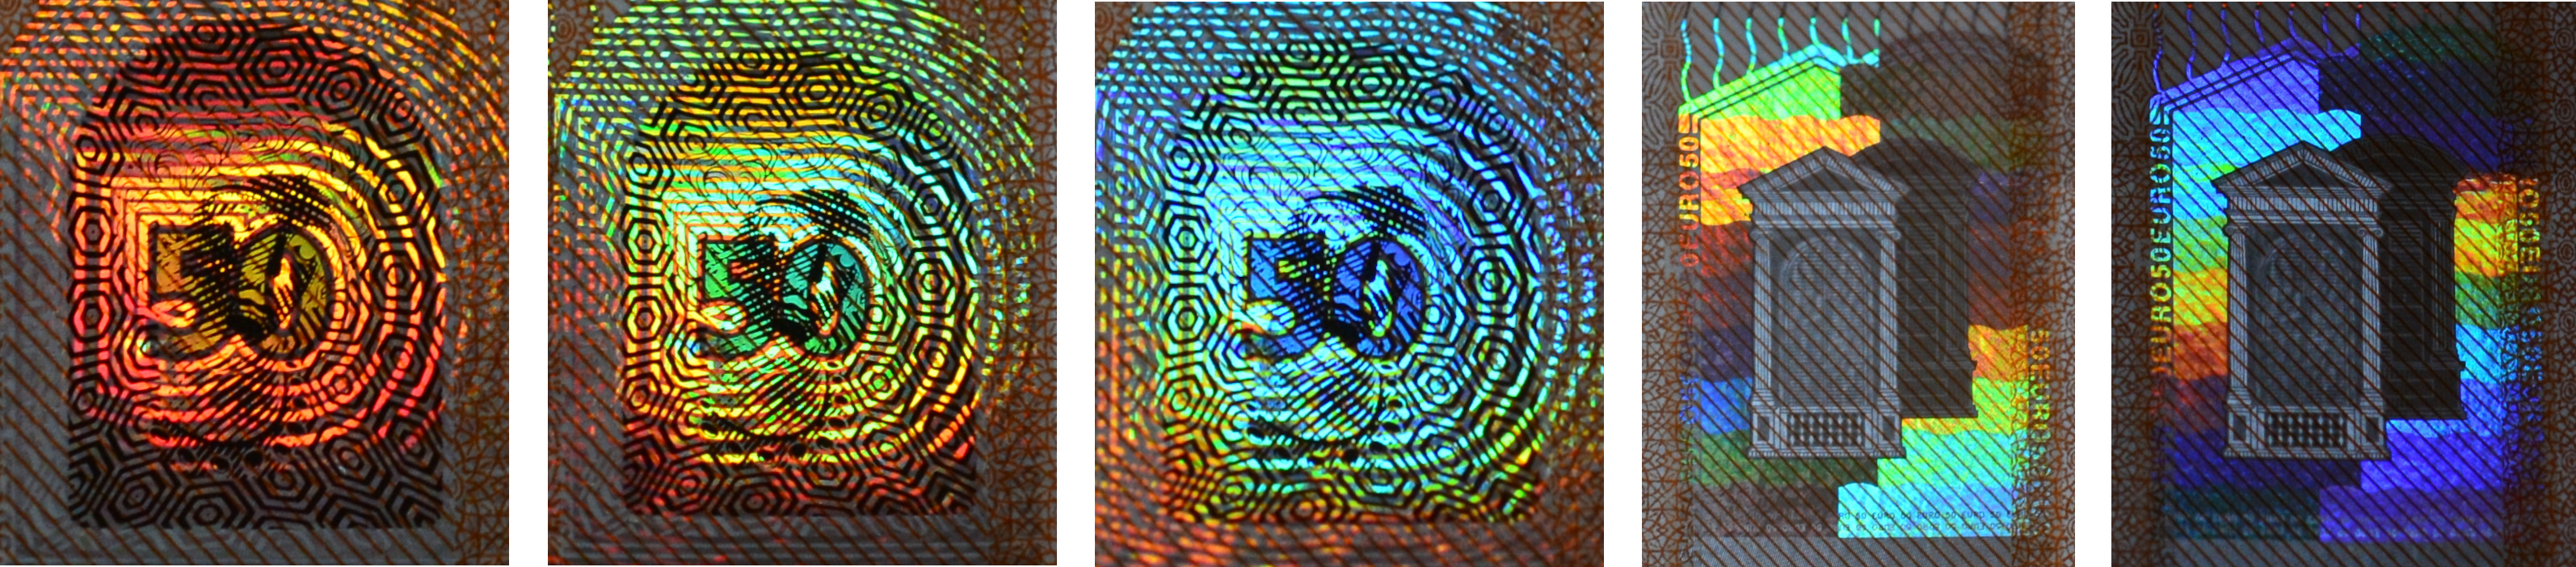
\includegraphics[width=13truecm]{slike/08_photo_hologram.jpg}
\caption{Holograma na evrskem bankovcu, kot ju vidimo pod različnimi koti. }
\label{fig:08_photo_hologram}
\vglue-10truemm
\end{figure}

\begin{remark}
Kadar zajamemo interferenco ne le v tankem filmu, temveč po debelejšem sloju, imenujemo 
nastalo interferenčno sliko volumski hologram. Za volumske holograme je značilno, da omogočajo 
opazovanje hologramov v naravnih barvah predmeta, kar dosežemo s posebnim tridimenzionalim zapisom 
v treh osnovnih barvah.
\end{remark}


